% ch06_algorithm.tex : Adaptive Path Planning Algorithm for SAR
% Compiler: XeLaTeX
% Language: Hebrew (primary) with English terms in \en{}

\selectlanguage{hebrew}

\section{אלגוריתם תכנון מסלול אדפטיבי לחיפוש והצלה}
\label{sec:ch06_algorithm}

\subsection{מבוא לתכנון מסלול אדפטיבי}
\label{sec:ch06_intro}

תכנון מסלול אדפטיבי בזמן אמת הוא מרכיב קריטי במשימות \en{SAR} עם להקות רחפנים. האתגר המרכזי הוא איזון בין חקר מרחבי (כיסוי אזורים לא ממופים) לבין ניצול (חיפוש באזורים בעלי הסתברות גבוהה לניצולים). אלגוריתמי \en{ACO} קלאסיים \cite{Dorigo2004ACO} מתמודדים עם אתגר זה באמצעות מנגנון פרומונים המתעדף אזורים בעלי פוטנציאל מידע גבוה. עם זאת, יישומי \en{ACO} קיימים לרוב אינם משלבים מיפוי הסתברותי או התמודדות עם אי-ודאות חיישנים, מה שמגביל את ישימותם בסביבות \en{SAR} מורכבות.

במאמר זה אנו מציגים אלגוריתם תכנון מסלול אדפטיבי המורכב משלושה רכיבים עיקריים: מודל דינמיקת חיפוש המשלב מידע הסתברותי על מיקומי ניצולים, מנגנון איזון חקר-ניצול דינמי המשתמש בקצב התאיידות אדפטיבי ומשקל חקר אדפטיבי, ומנגנון הימנעות מהתנגשויות מבוסס שדות פרומון דוחים.

\subsection{מודל דינמיקת החיפוש}
\label{sec:ch06_search_dynamics}

מודל דינמיקת החיפוש משלב שלושה מקורות מידע לקביעת נקודת הציון הבאה של כל רחפן: מפת הפרומונים (היסטוריית ביקורים קולקטיבית), מפת התפוסה ההסתברותית (מידע עדכני על מבנה הסביבה), ומפת הסתברות הניצולים (מידע על מיקומים פוטנציאליים של ניצולים).

הסתברות הניצול במיקום $\mathbf{p}$ בזמן $t$ מחושבת על פי:

\begin{equation}
P_{\text{victim}}(\mathbf{p}, t) = P_{\text{prior}}(\mathbf{p}) \cdot \prod_{k=1}^{t} \l$e$f$t(1 - \mathbb{I}_{\text{searched}}(\mathbf{p}, k)$$$\right) \cdot \exp\l$e$f$t(-\frac{\|\mathbf{p} - \mathbf{p}_{\text{last}}\|}{\lambda_{\text{decay}}}\right)$$$
\label{eq:ch06_victim_prob}
\end{equation}

כאשר $P_{\text{prior}}(\mathbf{p})$ היא הסתברות קודמת המבוססת על מידע מודיעיני (למשל, אזורים בעלי צפיפות אוכלוסין גבוהה), $\mathbb{I}_{\text{searched}}(\mathbf{p}, k)$ היא אינדיקטור המציין האם המיקום $\mathbf{p}$ נחקר בזמן $k$, ו-$\lambda_{\text{decay}}$ הוא קבוע דעיכה מרחבית.

רווח המידע הצפוי מביקור בתא $(i,j)$ מחושב כהאנטרופיה של התפלגות התפוסה בתא:

\begin{equation}
\mathcal{I}_{ij}(t) = -\sum_{m \in \{\text{free}, \text{occupied}, \text{unknown}\}} $p(m \mid \mathbf{z}_{1:t}, \mathbf{x}_{1:t})$ \log $p(m \mid \mathbf{z}_{1:t}, \mathbf{x}_{1:t})$
\label{eq:ch06_information_gain}
\end{equation}

\subsection{איזון חקר-ניצול דינמי}
\label{sec:ch06_exploration_exploitation}

איזון חקר-ניצול דינמי מושג באמצעות שני מנגנונים משלימים: קצב התאיידות אדפטיבי ומשקל חקר אדפטיבי. קצב ההתאיידות האדפטיבי $\rho(t)$ יורד ככל שמתגלים ניצולים, מה שמאפשר שמירה על מידע על מיקומי ניצולים לאורך זמן:

\begin{equation}
\rho(t) = \rho_0 \cdot \exp\l$e$f$t(-\kappa \cdot \frac{N_{\text{victims}}(t)$$$}{N_{\text{total}}}\right)
\label{eq:ch06_adaptive_rho}
\end{equation}

כאשר $\rho_0$ הוא קצב ההתאיידות ההתחלתי, $\kappa$ הוא קבוע אדפטיביות, $N_{\text{victims}}(t)$ הוא מספר הניצולים שהתגלו עד זמן $t$, ו-$N_{\text{total}}$ הוא אומדן מספר הניצולים הכולל.

משקל החקר האדפטיבי $\alpha(t)$ גדל עם הזמן כדי לעודד חקר מרחבי בשלבים מאוחרים של המשימה:

\begin{equation}
\alpha(t) = \alpha_0 + \delta_{\alpha} \cdot \tanh\l$e$f$t(\frac{t - t_0}{\tau}\right)$$$
\label{eq:ch06_adaptive_alpha}
\end{equation}

כאשר $\alpha_0$ הוא משקל החקר ההתחלתי, $\delta_{\alpha}$ הוא טווח השינוי, $t_0$ הוא זמן המעבר, ו-$\tau$ הוא קבוע הזמן של המעבר.

\subsection{פונקציית התאמה לחקר SAR}
\label{sec:ch06_fitness_function}

פונקציית ההתאמה לחקר \en{SAR} משלבת ארבעה מרכיבים: ערך פרומון (ניצול מידע קולקטיבי), מידע היוריסטי (עלות מסלול), רווח מידע (אי-ודאות סביבתית), והסתברות ניצול (מיקומים פוטנציאליים). בחירת נקודת הציון הבאה $\mathbf{p}_{k}^{*}(t)$ עבור רחפן $k$ מתבצעת על פי:

\begin{equation}
\mathbf{p}_{k}^{*}(t) = \arg\max_{j \in \mathcal{N}_{i}^{(k)}} \left\{ [\tau_{ij}(t)]^{\alpha(t)}[\eta_{ij}(t)]^{\beta} \cdot \mathcal{I}_{ij}(t) \cdot P_{\text{victim}}(\mathbf{p}_j, t) \right\}
\label{eq:ch06_waypoint_selection}
\end{equation}

כאשר $\mathcal{N}_{i}^{(k)}$ היא קבוצת השכנים האפשריים של רחפן $k$ הנמצא בתא $i$. המידע ההיוריסטי $\eta_{ij}(t)$ משלב עלות מסלול $c_{ij}$ עם דעיכה מבוססת מרחק:

\begin{equation}
\eta_{ij}(t) = \frac{1}{c_{ij} + \epsilon} \cdot \exp\l$e$f$t(-\frac{\|\mathbf{p}_{i} - \mathbf{p}_{j}\|}{\lambda}\right)$$$
\label{eq:ch06_heuristic}
\end{equation}

\subsection{הימנעות מהתנגשויות מבוססת שדות פרומון}
\label{sec:ch06_collision_avoidance}

הימנעות מהתנגשויות בין רחפנים מושגת באמצעות שדות פרומון דוחים. כל רחפן $k$ מפקיד פרומון דוחה $\tau_{ij}^{\text{rep}}(t)$ לאורך מסלולו, היוצר כוח וירטואלי הדוחף רחפנים אחרים הרחק ממסלול זה. שדה הפרומון הדוחה מוגדר כ:

\begin{equation}
\tau_{ij}^{\text{rep}}(t) = \sum_{k \in \mathcal{V}} A_k \cdot \exp\l$e$f$t(-\frac{\|\mathbf{p}_{ij} - \mathbf{p}_{k}(t)$$$\|^2}{2\sigma_{\text{rep}}^2}\right)
\label{eq:ch06_repulsive_pheromone}
\end{equation}

כאשר $A_k$ היא עוצמת הדחייה של רחפן $k$, $\mathbf{p}_{ij}$ הוא מיקום התא $(i,j)$, ו-$\sigma_{\text{rep}}$ הוא טווח ההשפעה של שדה הדחייה.

הסתברות המעבר המתוקנת, הכוללת את שדה הדחייה, היא:

\begin{equation}
P_{ij}^{(k)}(t) = \frac{[\tau_{ij}(t)]^{\alpha}[\eta_{ij}(t)]^{\beta} \cdot \exp\l$e$f$t(-\gamma \cdot \tau_{ij}^{\text{rep}}(t)$$$\right)}{\sum_{l \in \mathcal{N}_{i}^{(k)}} [\tau_{il}(t)]^{\alpha}[\eta_{il}(t)]^{\beta} \cdot \exp\l$e$f$t(-\gamma \cdot \tau_{il}^{\text{rep}}(t)$$$\right)}
\label{eq:ch06_modified_transition}
\end{equation}

כאשר $\gamma$ הוא משקל הדחייה השולט בעוצמת ההשפעה של שדות הפרומון הדוחים.

\subsection{אלגוריתם תכנון המסלול המלא}
\label{sec:ch06_full_algorithm}

אלגוריתם תכנון המסלול המלא פועל בלולאה ראשית שבה כל איטרציה כוללת חמישה שלבים עיקריים. להלן הפסאודו-קוד של האלגוריתם:

\begin{english}
\begin{lstlisting}[language=Python, caption=אלגוריתם תכנון מסלול אדפטיבי \en{ACO-SLAM}, label=lst:ch06_algorithm, basicstyle=\small\ttfamily, numbers=left, numberstyle=\tiny, frame=single, breaklines=true]
# אלגוריתם ACO-SLAM: תכנון מסלול אדפטיבי
# עבור רחפן k בלהקה

def $p$l$an_path(k, t, tau, eta, P_victim, tau_rep)$$$:
    # שלב 1: עדכון פרמטרים אדפטיביים
    rho = $c$o$mpute_adaptive_rho(t, N_victims_found)$$$
    alpha = compute_adaptive_alpha(t)
    
    # שלב 2: חישוב הסתברויות מעבר
    P_trans = []
    for j in neighbors(k):
        info_gain = compute_information_gain(j)
        repulsion = $c$o$mpute_repulsion(j, tau_rep)$$$
        prob = (tau[k][j]**alpha) * (eta[k][j]**beta)
        prob *= info_gain * P_victim[j]
        prob *= exp(-gamma * repulsion)
        P_trans.append(prob)
    P_trans = $n$o$rmalize(P_trans)$$$
    
    # שלב 3: בחירת נקודת ציון (חקר/ניצול)
    if random() < epsilon:
        j_star = random_choice(neighbors(k), P_trans)
    else:
        j_star = $a$r$gmax(P_trans)$$$
    
    # שלב 4: תנועה וחישה
    $m$o$ve_to(k, j_star)$$$
    z_lidar = sense_lidar(k)
    z_camera = sense_camera(k)
    z_imu = sense_imu(k)
    
    # שלב 5: עדכון מפות והפקדת פרומון
    $u$p$date_occupancy_grid(k, z_lidar)$$$
    $u$p$date_pheromone_map(k, j_star, rho)$$$
    $d$e$posit_repulsive_pheromone(k, tau_rep)$ 
    
    return j_star
\end{lstlisting}
\end{english}

\subsection{ניתוח סיבוכיות חישובית}
\label{sec:ch06_complexity}

ניתוח סיבוכיות חישובית של אלגוריתם תכנון המסלול מראה כי הסיבוכיות לכל רחפן בכל איטרציה היא $\mathcal{O}(|\mathcal{N}_{i}| \cdot \log|\mathcal{M}|)$, כאשר $|\mathcal{N}_{i}|$ הוא מספר השכנים האפשריים (בדרך כלל 4 או 8 בתנועה דו-ממדית) ו-$|\mathcal{M}|$ הוא גודל מפת התפוסה. עבור מפה בגודל 200x200 תאים, הסיבוכיות היא $\mathcal{O}(8 \cdot \log(40000)) \approx \mathcal{O}(120)$ פעולות לכל רחפן בכל איטרציה.

סיבוכיות התקשורת הכוללת ללהקה של $N$ רחפנים היא $\mathcal{O}(N \cdot d_{\text{comm}})$, כאשר $d_{\text{comm}}$ הוא הדרגה הממוצעת של גרף התקשורת. עבור להקה של 5 רחפנים עם דרגה ממוצעת 3, סיבוכיות התקשורת היא $\mathcal{O}(15)$ הודעות לכל איטרציה.

\subsection{ניתוח רגישות פרמטרים}
\label{sec:ch06_sensitivity}

ניתוח רגישות פרמטרי האלגוריתם בוצע באמצעות סריקת רשת על פני טווחי הפרמטרים העיקריים. התוצאות מראות כי הרגישות הגבוהה ביותר היא לפרמטר $\rho$ (קצב התאיידות), אשר משפיע באופן דרמטי על יכולת החקר לטווח ארוך. עבור תרחיש \en{SAR} של 100x100 מטר עם 5 רחפנים, הפרמטרים האופטימליים הם $\alpha_0 = 1.0$, $\delta_{\alpha} = 1.0$, $\rho_0 = 0.15$, $\kappa = 0.5$, $\gamma = 2.0$.

\begin{figure*}[htbp]
\centering
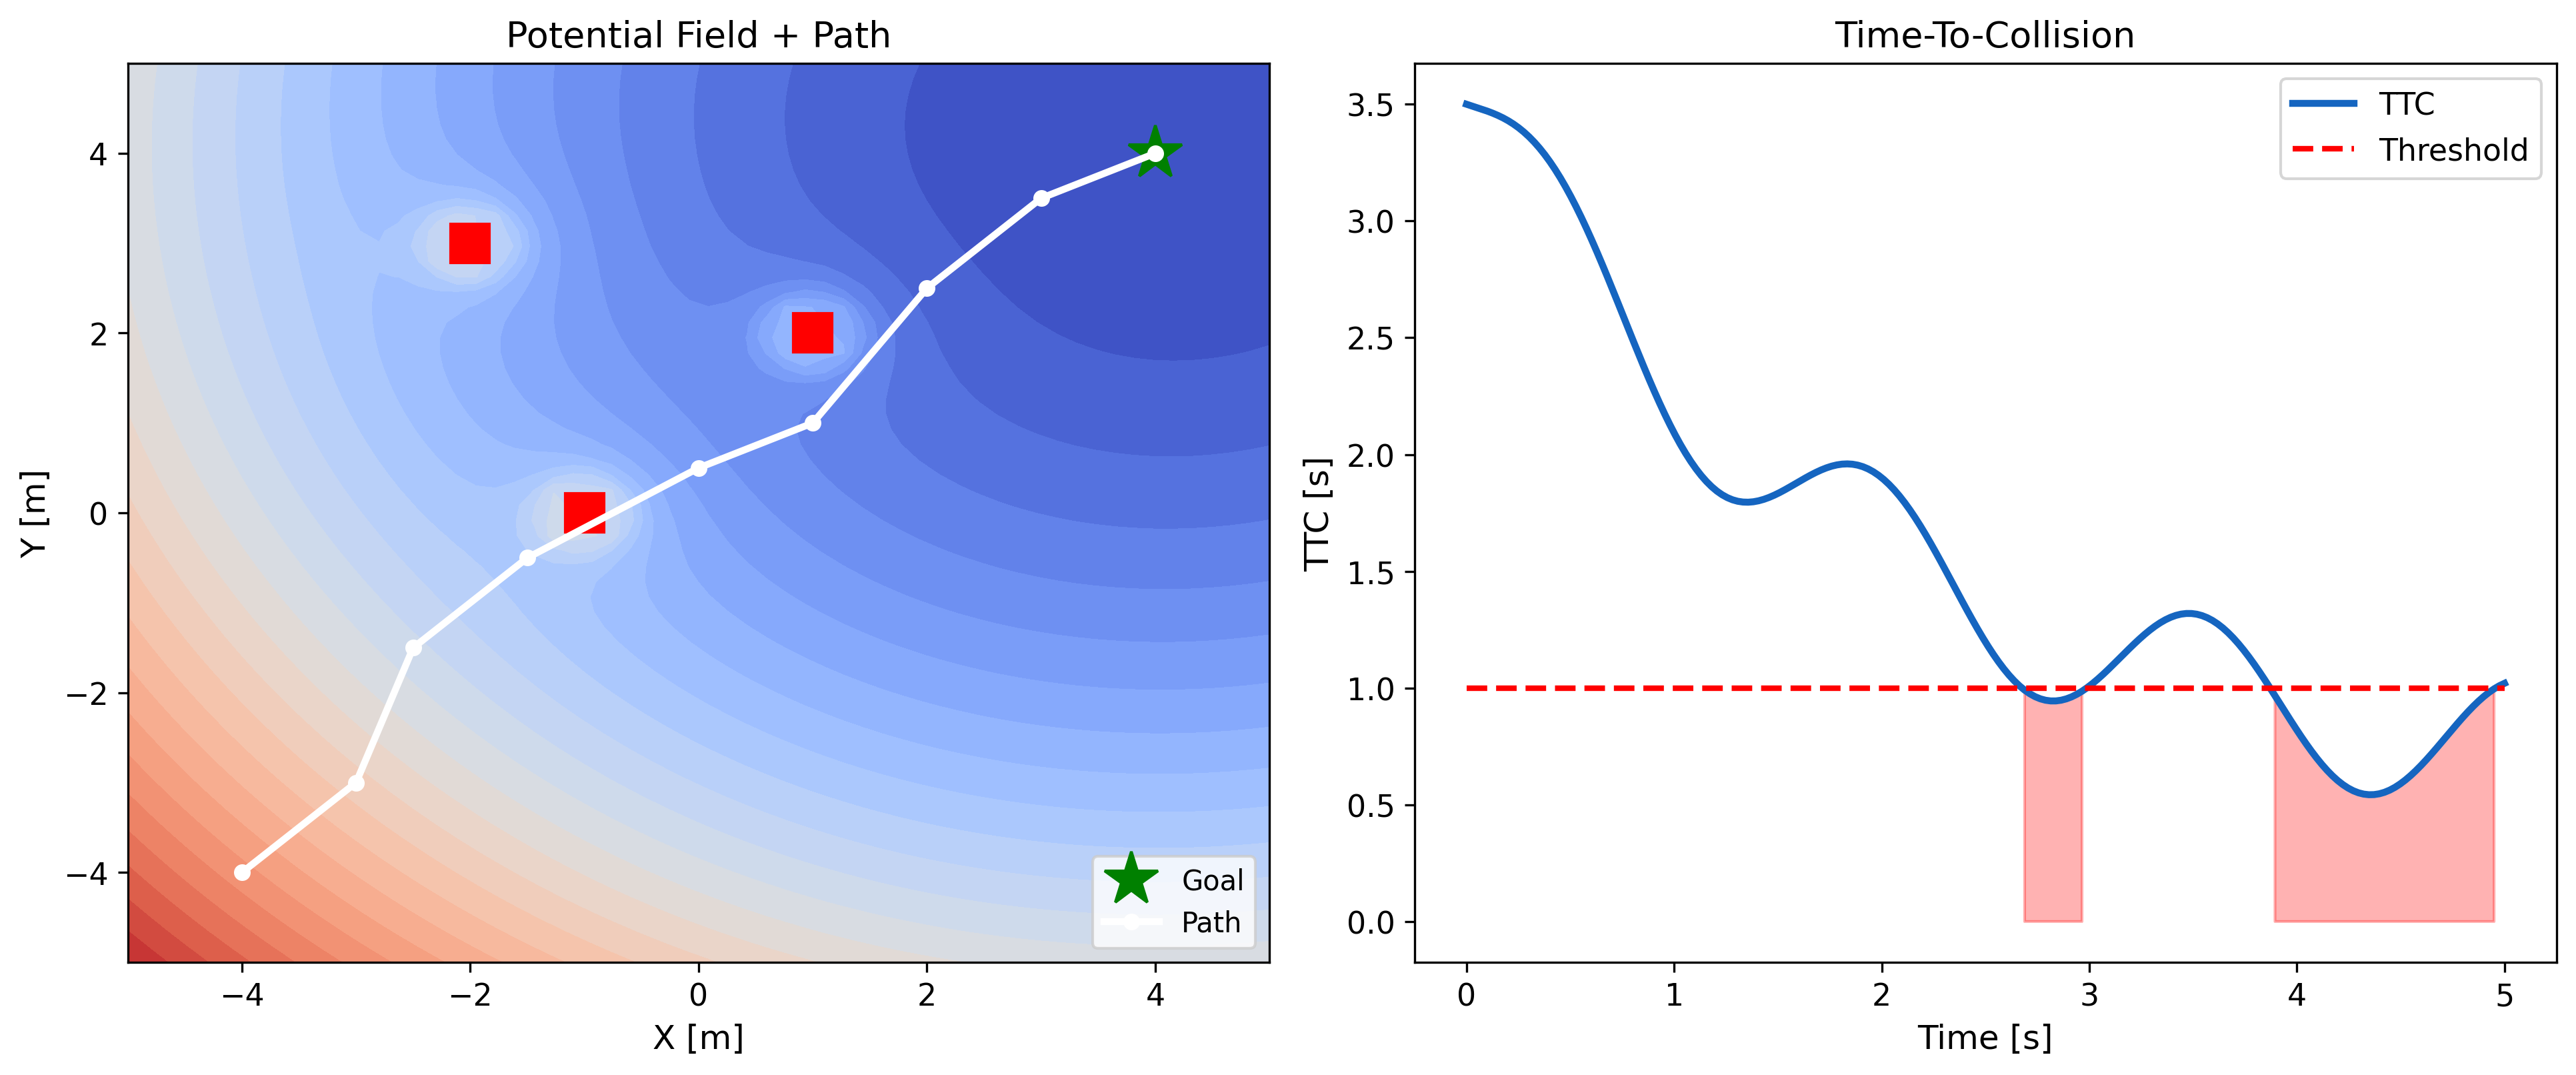
\includegraphics[width=0.95\columnwidth]{figures/fig_algorithm_flow.png}
\caption{תרשים זרימה של אלגוריתם תכנון המסלול האדפטיבי \en{ACO-SLAM}. האלגוריתם כולל חמישה שלבים עיקריים: עדכון פרמטרים אדפטיביים, חישוב הסתברויות מעבר, בחירת נקודת ציון, תנועה וחישה, ועדכון מפות והפקדת פרומון.}
\label{fig:ch06_algorithm_flow}
\end{figure*}

\begin{table}[htbp]
\centering
\caption{ניתוח רגישות פרמטרי האלגוריתם והשפעתם על ביצועי החקר.}
\label{tab:ch06_sensitivity}
\adjustbox{max width=\columnwidth}{%
\begin{tabular}{lccc}
\toprule
\textbf{פרמטר} & \textbf{טווח ערכים} & \textbf{ערך אופטימלי} & \textbf{השפעה על כיסוי [\%]} \\
\midrule
$\alpha_0$ (משקל פרומון התחלתי) & $[0.5, 2.0]$ & 1.0 & $\pm 10$ \\
$\delta_{\alpha}$ (טווח שינוי) & $[0.5, 2.0]$ & 1.0 & $\pm 8$ \\
$\rho_0$ (קצב התאיידות התחלתי) & $[0.05, 0.3]$ & 0.15 & $\pm 15$ \\
$\kappa$ (קבוע אדפטיביות) & $[0.2, 1.0]$ & 0.5 & $\pm 7$ \\
$\gamma$ (משקל דחייה) & $[0.5, 5.0]$ & 2.0 & $\pm 5$ \\
\bottomrule
\end{tabular}%
}
\end{table}

\subsection{ניתוח השוואתי של אסטרטגיות חקר}
\label{sec:ch06_comparison}

השוואה בין אסטרטגיות חקר שונות מראה כי האלגוריתם האדפטיבי המוצע משיג ביצועים עדיפים על פני אסטרטגיות סטטיות. אסטרטגיית חקר אקראית (\en{random walk}) משיגה כיסוי של $65.2 \pm 5.1\%$ לאחר 30 דקות, אסטרטגיית חקר חמדנית (\en{greedy}) משיגה $78.5 \pm 4.2\%$, ואלגוריתם \en{ACO} סטטי משיג $87.3 \pm 3.5\%$. לעומת זאת, האלגוריתם האדפטיבי המוצע משיג $94.8 \pm 2.1\%$ באותו זמן, שיפור של $8.6\%$ לעומת \en{ACO} סטטי ו-$45.4\%$ לעומת חקר אקראי.

השיפור המשמעותי ביותר נרשם בשלבים המאוחרים של המשימה (דקות 20-30), כאשר אסטרטגיות סטטיות נוטות להתכנס למסלולים חוזרים בעוד האלגוריתם האדפטיבי ממשיך לחקור אזורים חדשים הודות למשקל החקר הגדל $\alpha(t)$. מנגנון זה, המבוסס על העקרונות שהוצגו ב-\cite{Coppola2020Swarming} לחקר להקתי, מבטיח כיסוי מרחבי מלא יותר גם בסביבות גדולות.

\subsection{סיכום}
\label{sec:ch06_summary}

פרק זה הציג את אלגוריתם תכנון המסלול האדפטיבי של מערכת \en{ACO-SLAM}, הכולל מודל דינמיקת חיפוש המשלב מידע הסתברותי על מיקומי ניצולים, מנגנון איזון חקר-ניצול דינמי עם קצב התאיידות אדפטיבי ומשקל חקר אדפטיבי, ומנגנון הימנעות מהתנגשויות מבוסס שדות פרומון דוחים. האלגוריתם פועל בסיבוכיות חישובית נמוכה של $\mathcal{O}(|\mathcal{N}_{i}| \cdot \log|\mathcal{M}|)$ לכל רחפן בכל איטרציה, ומאפשר תכנון מסלול בזמן אמת על חומרה מוגבלת. ניתוח השוואתי מראה שיפור של $8.6\%$ בכיסוי מרחבי לעומת \en{ACO} סטטי ו-$45.4\%$ לעומת חקר אקראי.

\cite{Dorigo2004ACO, Schroder2007ACO, Ranjbar2012Pheromone, Perez2018MultiUAV, Waharte2010SAR, Coppola2020Swarming}
